%% ドキュメントクラスのロード jarticle クラス
%% onecolumn : 一段組み
%% a4j : A4サイズ,和文
%% fleqn : 数式は左揃え
\documentclass[10.5pt,twocolumn,a4j,fleqn]{ujarticle}

%% 使用パッケージの指定
%% graphicx : 図の使用
%% fancyhdr : ヘッダ設定
%% lastpage : ページ番号出力マクロ
\usepackage[dvipdfmx]{graphicx}
\usepackage{fancyhdr}
\usepackage{lastpage}
\usepackage{listings, jlisting}
\usepackage{bm}
\usepackage{mathptmx}
\usepackage{amsmath}
\usepackage{amsfonts}
\usepackage{amsmath}
\usepackage[subrefformat=parens]{subcaption}
\usepackage{geometry}
\usepackage{tabularx}

\lstset{
  numbers=left,
  numbersep=-10pt,
  columns=l
}
%ページの余白設定--------------------------------------------------
\geometry{left=15mm, right=15mm, bottom=20mm}

%自作コマンド--------------------------------------------------
%% 独自マクロ タイトルスタイルの変更
\makeatletter
\let\@oldmaketitle=\@maketitle
\def\@maketitle{
  \vskip -3zh
  \@oldmaketitle
  %\vspace*{-0.8cm}
}
\makeatother

%% 参照
\def\figref#1{図\ref{#1}}
\def\tblref#1{表\ref{#1}}
\def\eqref#1{式(\ref{#1})}
%----------------------------------------------------------------

%% ページのレイアウト指定
\setlength{\textheight}{242mm}
\setlength{\mathindent}{1zw}
\setlength{\headheight}{15.0pt}
\setlength{\voffset}{-1cm}

%% ヘッダスタイルの適用
\pagestyle{fancy}
\lhead{ 大学院-輪講 \today{}}
\chead{}
\rhead{}
\lfoot{}
\cfoot{\thepage}
\rfoot{}
\renewcommand\headrulewidth{0.4pt}
\renewcommand\footrulewidth{0pt}


\title{
    {\Large{\bf Monocular template-based reconstruction of inextensible surfaces  \cite{Perriollat2011}}}
}
\author{\bf{
        \input{name.tex}
    }\\
}
\date{}

%%----- ここから論文本体 ---------------------------------------
\begin{document}
\maketitle

\section{ざっくり概要}\label{sec1}
\subsection{アブストラクト}
平面テンプレートを利用した,点対応を用いて非伸縮な物体の表面形状を再構成する.
非伸縮とは,物体表面が伸び縮みしないことをいい,例えば,紙のような柔軟物体に相当する.
本研究では,まず,Pointwise法:3D点の対応を回復する方法を提案した.
この手法は3次元点の誤差を扱い,SOCP(Second-Order Cone Program)として定式化される.
Pointwise法は,3次元表面の点間のユークリッド距離が測地線の長さよりも短いことに依存する.
また,再構成の平滑化手法を提案した.この手法は,FFD(Free-Form Deformations)を用いてなめらかな表面を再構成する.
平滑な表面は,2次元の点から3次元点へのマッピングによって表現される.
この時,2D-3Dマップは,どこでも局所的にアイソメトリ(isometry)であるとする.この仮定により,
表面形状の最適化問題がマップのヤコビ行列で表現され,最小二乗法最小化問題として解くことができる.

\subsection{結論}
単眼カメラを用いた,非伸縮な表面形状推定手法を提案した.
\begin{enumerate}
    \item Pointwise法を用いて再構成した3次元点の深度を最大化する凸コスト関数としてSOCPに落とし込み,再構成誤差を改善した.
    \item FFDベースの平滑化手法により再構成表面が従来手法よりも精度が高くなった.
    \item 実験によって再構成表面は確かに非伸張性を持つことをしめした.
    \item 最適解に近い初期解を構築することにより,SOCP,FFDの非凸コスト関数の非線形最小化問題を解消した.
\end{enumerate}
\subsection{本研究で扱う変数について}
\tblref{table1}にて本研究で使用する変数を定義しておく.


\begin{table}[htb]
  \caption{変数の説明}
  \begin{tabular}{|c|l|} \hline
    Notation & Description \\ \hline
    $\bm{P}$ & カメラの内部パラメータ,$\bm{P} \in \mathbb{R}^{3\times3}$  \\
    $\bm{p}_k^{\mathrm{T}}$ & カメラの内部パラメータ行列の k行目  \\
    $n_c$ & 点対応組の総数 \\
    $\bm{q}_i$ & テンプレート画像平面内のi番目の点 $i \in {1, ... ,n_c}$ \\
    $\bm{q}_i^{\prime}$ & 入力画像平面内のi番目の点 \\
    $\overline{\bm{q}}_i$ & 点$\bm{q}_i$の同時座標系 \\
    $\bm{u}_i$ & 点$\bm{q}_i^{\prime}$ に関する視線,$\bm{u}_i = (\bm{P^{-1}} \bm{q}_i^{\prime}) / \| \bm{P^{-1}} \bm{q}_i^{\prime} \|)$ \\
    $\bm{Q}_i$ & 再構成された3次元点 \\
    $\mu_i$ & 点$\bm{Q}_i$ の深度 \\
    $d_{ij}$ & 点$i, j$間のユークリッド距離,$(d_{ij} = \|\bm{q}_i - \bm{q}_j\|)$ \\
    $\hat{x}$ & 値$x$の真値,($x = \bm{q}_i^{\prime}, \bm{q}_i, \bm{Q}_i, \bm{u}_i, \mu_i, d_{ij}$) \\ \hline
  \end{tabular}
  \label{table1}
\end{table}


\subsection{実験結果}
\subsubsection{人工データにおける実験}
\figref{fig2}に実験で用いたデータを示す.左が3次元表面である.中央は,テンプレート画像である.右は実験の入力画像である.青い点はランダムに生成した,点の対応組である.
オブジェクトは$ 20 mm $ の大きさである.仮想カメラはオブジェクトから約 $1m$ の位置にある.
また,仮想カメラのフォーカルレングス(focal length)は $36mm$ とした.2D-3D対応点組 $n_c$ は表面上にランダムに生成される.
さらに,3次元表面の点には標準正規分布に従うノイズを使用した.
このとき,分布の分散 $\sigma = 1$ pixelとした.

\begin{figure*}[htbp]
 \begin{center}
  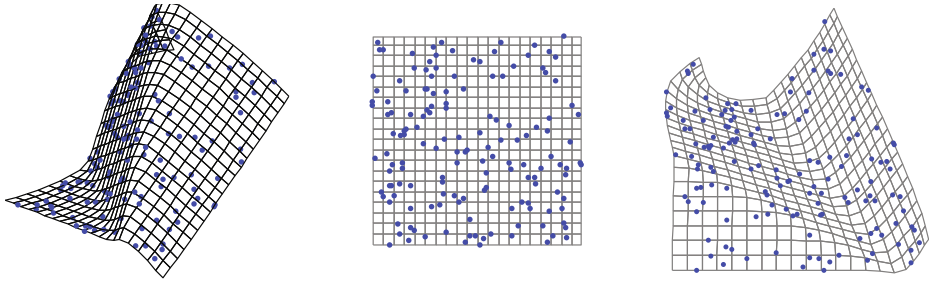
\includegraphics[width=150mm]{img/fig2.png}
  \caption{実験で用いたデータ}
  \label{fig2}
 \end{center}
\end{figure*}

実験では,本手法と関連するアルゴリズムを比較した.
\begin{description}
    \item[SOCPimg]\mbox{}\\ 
        項\ref{sec:socp}で示したPointwiseアルゴリズム
    \item[FFDref]\mbox{}\\
        項\ref{sec:FFDref}で示した平滑な再構成アルゴリズム
    \item[FFDinit]\mbox{}\\
        再構成アルゴリズムによる初期解
    \item[Salz]\mbox{}\\
        凸関数を用いた手法でSOCPによる定式化の際のノイズの扱いが,提案手法と異なる \cite{Salzmann2009}.ノイズを処理するために,再投影誤差を含むコスト関数を最小化する手法を提案している.
    \item[PerrioInit]\mbox{}\\
        `upper depth bound' 法である\cite{Perriollat2011a}. これはpointwiseアルゴリズムであるが,逐次,非伸張性の拘束条件適用する.
    \item[PerrioRef]\mbox{}\\
        \cite{Perriollat2011a}の改良手法.PerrioInitよりも良い再構成結果が得られる.
\end{description}

\paragraph{実験1:再構成エラー}
表面の真値と比較し,異なる手法の比較を行うために,本稿では,Pointwise reconstruction error(PWRE)を次式で定義した.
\begin{equation}
    e_p = \frac{1}{n_c} \sum_{i=1}^{n_c}  \| \bm{Q}_i - \hat{\bm{Q}}_i\|
\end{equation}
また,FFDや三角メッシュを用いるような複雑なアルゴリズムに対しては,Surface Reconstruction Error(SRE)を次式で定義した.
\begin{equation}
    e_s =  \iint \| \mathcal{W}_{\bm{\ell}} - \hat{\mathcal{W}}(\bm{q}) \| d\bm{q}
\end{equation}
この実験では, $1,000$ 個のランダムな形状をしたメッシュシートを生成した.また,点対応組は $n_c = 150$ とした.
\figref{fig3a}に全てのアルゴリズムのPWREの結果を示している.そして\figref{fig3b}にはSREを示している.
本稿で提案した最終的な再構生{\bf FFDref}は,PWRE,SREともに最小値となった.
全体的に,複雑表面モデルを用いたアルゴリズムが,pointwise法と比較してエラーが小さい結果となった.
\begin{figure}[htbp]
  \begin{minipage}[t]{\hsize}
    \centering
    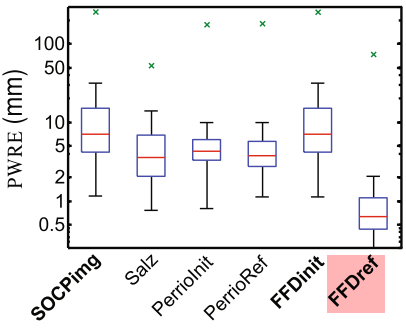
\includegraphics[width=\linewidth]{img/fig3a.png}
    \subcaption{PWREの結果}
    \label{fig3a}
  \end{minipage}
    \\
  \begin{minipage}[t]{\hsize}
    \centering
    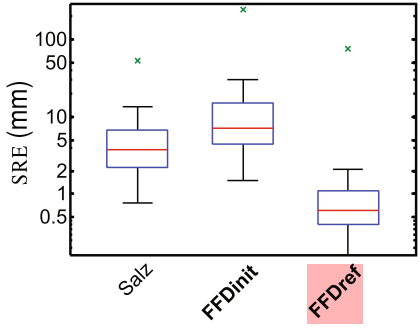
\includegraphics[width=\linewidth]{img/fig3b.png}
    \subcaption{SREの結果}
    \label{fig3b}
  \end{minipage}
 \caption{再構成エラーの比較}
\end{figure}

\paragraph{実験2:測地線の長さ}
ここでは,本提案手法が再構成した表面が非伸張性を持つことを実験によって示す.
実験に使用した表面データは前の実験と同じものを使う.
テンプレート上の点は$10,000$個ランダムに生成した.
全ての点の組$(\bm{g}_i,\bm{g}_j)$ について,測地線の長さ $l_{ij}^{3D}$ は,
表面上の頂点$ \mathcal{W}_{\bm{\ell}}(\bm{g}_i)$ と $ \mathcal{W}_{\bm{\ell}}(\bm{g}_j)$
で変形表面に沿って結ばれる線分の長さである.
ただし,測地線は次式で2点を結ぶ折れ線で近似できる.

\begin{equation}
    l_{ij}^{3D} = \sum_{k=1}^{n_g} \| \mathcal{W}_{\bm{\ell}}(\bm{g}_i + \frac{k}{n_g}\|\bm{g}_j - \bm{g}_i\|) -  \mathcal{W}_{\bm{\ell}}(\bm{g}_i + \frac{k-1}{n_g}\|\bm{g}_j - \bm{g}_i\|)\|
\end{equation}

$n_g$ は折れ線近似で用いた中間点の数である.本研究では,実験的に安定した中間点数$n_g$ が 180以上であるとき安定することがわかっているので,$n_g = 200$ とした.
\figref{fig4a}に{\bf FFDinit}の比較と,\figref{fig4b},\figref{fig4c}に{\bf FFDref}の比較を示す.
{\bf FFDref}のグラフから,提案手法によって再構成した表面の測地線の長さとテンプレート平面の線分の距離がほとんど等しい結果を得た.
すなわち,{\bf FFDref}の再構成結果は確かに非伸張性を持った表面であることを示している.
対して,本稿の提案した初期解{\bf FFDinit}のグラフ\figref{fig4a}は疎な結果であり,非伸張性を持つとは言えない.
\begin{figure}[htbp]
    \centering
  \begin{minipage}[t]{\hsize}
    \centering
    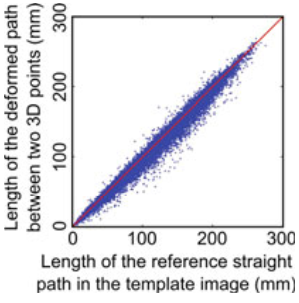
\includegraphics[width=0.7\linewidth]{img/fig4a.png}
    \subcaption{FFDinit}
    \label{fig4a}
  \end{minipage}
    \\
  \begin{minipage}[t]{\hsize}
    \centering
    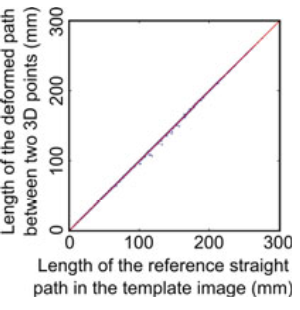
\includegraphics[width=0.7\linewidth]{img/fig4b.png}
    \subcaption{FFDref}
    \label{fig4b}
  \end{minipage}
    \\
  \begin{minipage}[t]{\hsize}
    \centering
    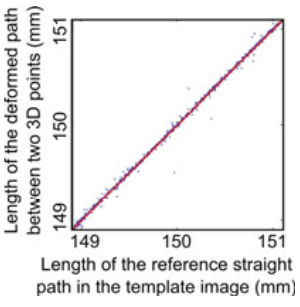
\includegraphics[width=0.7\linewidth]{img/fig4c.png}
    \subcaption{図\ref{fig4b}の拡大図}
    \label{fig4c}
  \end{minipage}
 \caption{非伸張性の証明}
\end{figure}
また,テンプレート平面上の点$\bm{g}_i,\bm{g}_j$間のユークリッド距離を$l_{ij}^{2D}$として,\tblref{table2}に誤差$l_{ij}^{2D}/l_{ij}^{3D}$の統計的評価を示した.
\begin{table*}[htb]
  \caption{測地線の実際の誤差}
  \centering
  \begin{tabular}{|r|r|r|r|r|r|} \hline
      & Mean & Std. deviation & Median & Mininum & Maximum \\ \hline
      FFDinit& 0.0119 & 0.0417 & 0.0036 & -1.9689 & 0.8931 \\ \hline
      FFDref& $2.0084\times1-^{-5}$ & $7.1965\times10^{-4}$ & $5.8083\times10^{-6}$ & -0.0505 & 0.3396 \\ \hline
  \end{tabular}
  \label{table2}
\end{table*}


\paragraph{実験3:ガウス曲率}
表面における2方向の主曲率の積をガウス曲率という.ガウス曲率が0の時,その面は非伸縮である.
非伸縮な表面形状のガウス曲率は通常ゼロであることから,提案手法によって再構成した表面がガウス曲率がゼロであることを実験によって示した.
再構成した表面上の点10,000点のガウス曲率を計算した.
\tblref{table3}に実験結果を示す.{\bf FFDref}は統計処理に従って得た平均値はゼロに近く,ほとんど非伸縮な表面形状である.また{\bf FFDinit}よりも{\bf FFDref}は100倍小さくなった.
\begin{table*}[htb]
  \caption{ガウス曲率による提案手法の非伸長性評価}
  \centering
  \begin{tabular}{|r|r|r|r|r|r|} \hline
      & Mean & Std. deviation & Median & Mininum & Maximum \\ \hline
      FFDinit& $4.9458\times10^{-4}$ & 0.0875 & $9.7302\times10^{-5}$ & $7.5122\times10^{-14}$ & 258.2379 \\ \hline
      FFDref& $5.0046\times1-^{-6}$ & $7.1320\times10^{-4}$ & $1.7333\times10^{-6}$ & $2.2325\times10^{-14}$ & 1.5199 \\ \hline
  \end{tabular}
  \label{table3}
\end{table*}

\subsubsection{実環境}
\figref{fig5}にオクルージョンありの実験結果を示す.
提案手法{\bf FFDref}は他の手法と比較して,オクルージョンにより対応点がない場合でも,表面全体で非伸張性を保ち,再構成されている.
\begin{figure*}[htbp]
 \begin{center}
  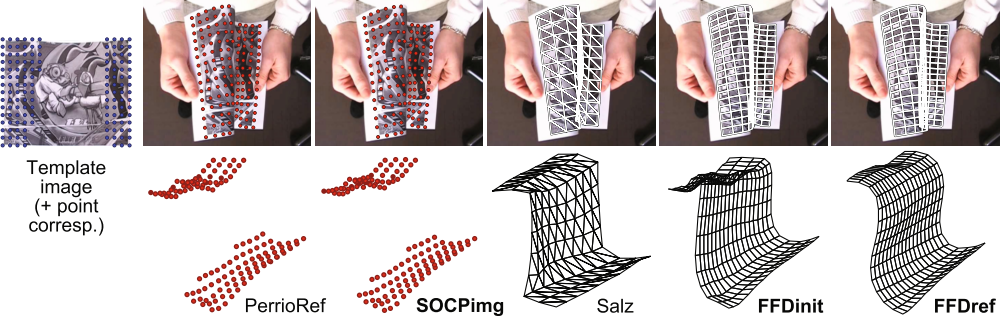
\includegraphics[width=150mm]{img/fig5.png}
  \caption{オクルージョンありの表面形状推定結果}
  \label{fig5}
 \end{center}
\end{figure*}

さらに,\figref{fig6}にステレオ再構成によって得られた正確な再構成結果と比較している.
\tblref{table4}に,正確な3次元表面と各手法の3次元エラーを比較した結果を示す.
\figref{fig6}の1行目は,入力画像と推定表面を合成した画像である.2行目は,
再構成した3次元表面を異なる視点から見た図である.ただし,最初の列がステレオアルゴリズムによって再構成した結果である.
\tblref{table4}より,ステレオアルゴリズムの3次元表面と比較して3次元エラーの平均が最も小さいものは,提案手法の{\bf FFDref}であった.


\begin{figure*}[htbp]
 \begin{center}
  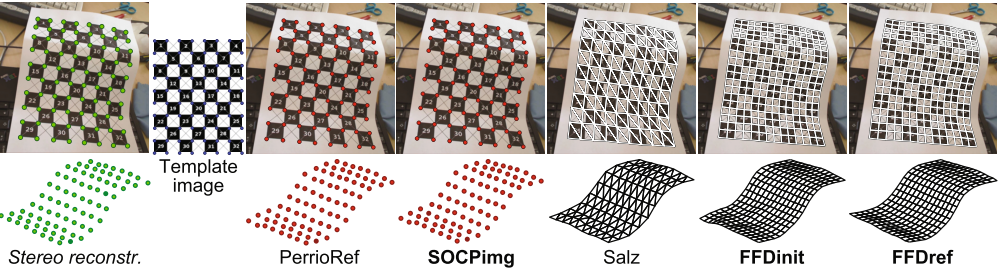
\includegraphics[width=150mm]{img/fig6.png}
  \caption{ステレオ法と各手法による3次元表面の再構成結果}
  \label{fig6}
 \end{center}
\end{figure*}

\begin{table}[htb]
  \begin{tabular}{|r|r|r|r|r|} \hline
    PerrioRef & SOCPimg & Salz & FFDinit & FFDref \\ \hline
    2.388 & 2.261 & 4.743 & 2.259 & {\bf 1.991} \\ \hline
  \end{tabular}
  \caption{ステレオ法に対する3次元エラーの平均(mm)}
  \label{table4}
\end{table}

\section{関連研究}
変形可能な表面の3次元再構成の研究において,紙のような変形物体が伸縮しないと仮定することは一般的である.
非伸縮性表面を有するとは、表面が基準形状の等長性変形であることを意味する.
すなわち,いかなる変形も,変形面上の点間の測地線の長さが不変であるといえる.
しかし,この非伸張性を再構成アルゴリズムに組み込むことは難しい.
実際,表面が三角メッシュや疎な点のメッシュで湾曲面が表現される場合,測地線を求めることは難しい.
以上の理由から,近似手法が提案されてきた.

第一の近似手法について述べる.これは,表面が極端に曲がらない形状であると仮定した時,ユークリッド距離が測地線の近似に有効である.
ただし,この制約条件は拘束力が弱い.ユークリッド距離が測地線から大きく逸れないことを前提としている.
また,この近似手法は点が十分にある場合に有効である.しかし,表面モデルによっては,制御点の数を変更することが必ずしも可能でない.
さらに,2次元の場合うまく行く場合があるが,3次元表面の場合はほとんどうまく行かない.
これは,\figref{fig1}に示すとおり,3次元表面上の点$\bm{Q}_i$のユークリッド距離に対して測地線$d_{ij}$は長いことがわかる.
そこで,古典的手法としてよく知られているのが`upper bound paaroach'である.
これは,3次元空間の2点間のユークリッド距離が小さくなっても,表面上の測地線の長さよりも大きくならないことを意味する.
これを非伸張制約$\| \bm{Q}_i -\bm{Q}_j\| \le d_{ij}$と表せる.
また,3次元点$\bm{Q}_i$は,カメラの視線ベクトル$\mathrm{\bm{u}}_i$と深度$\mu_i$ によって $\bm{Q}_i =\mu_i \mathrm{\bm{u}}_i$と表せる.
すなわち,深度が定まらないため,再構成を困難にする要因である.
この問題を解決する手法として,ヒューリスティック法がある.これは,再構成した3次元点の深度を最大化する.

また,異なる手法も提案されている\cite{Perriollat2011a}.非伸張性制約条件を組み込み,テンプレート画像のノイズを説明したアルゴリズムである.
ノイズとは測地距離に対して与える小さな値である.すなわち,非伸張性制約条件に対して,$d_{ij}$はテンプレート画像内の最大ノイズ$\varepsilon_{\mathcal{T}}$
によって書き換えられる.$d_{ij} + \varepsilon_{\mathcal{T}}$

また,\cite{Salzmann2009}によって別の手法も提案されている.
彼らのアプローチは,負数の再投影誤差と再構成された3d点の深度を最大化する凸面のコスト関数を使う.このときの制約式は非伸長性の不等式である.
この問題はSOCPとして容易に解くことが可能である.

\begin{figure*}[htbp]
 \begin{center}
  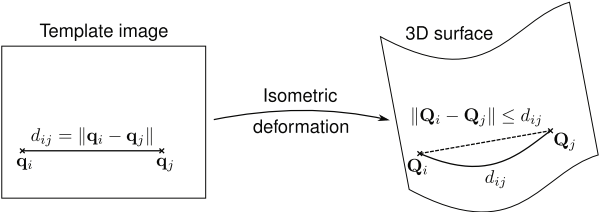
\includegraphics[width=150mm]{img/fig1.png}
  \caption{表面上の点および線分と点どうしのユークリッド距離}
  \label{fig1}
 \end{center}
\end{figure*}

\section{Upper Bound Approachの凸関数} \label{sec:socp}
本研究ではpointwise法を用いることで,再投影誤差の最小化と深度の最大化の相対的な影響を調整することを回避し,凸関数(comvex formulation)をSOCP問題として定式化する.
先に述べた非伸張性制約条件に対して,3次元表面についても制約を加える事を考える.
入力画像平面上の距離に関して非伸張性制約条件を,最大エラー$\varepsilon_{\mathcal{I}}$を考えると,

\begin{equation}
    \| \hat{\bm{q}}_i^{\prime} - \bm{q}_i^{\prime}\| \le \varepsilon_{\mathcal{t}}
\end{equation}
今,3次元点$\bm{Q}_i$について考えるので,真値$\hat{\bm{q}}_i^{\prime}$は,
\begin{equation}
    \hat{\bm{q}}_i^{\prime} = \frac{1}{\mathrm{\bm{p}}_3^{\mathrm{T}} \bm{Q}_i} \left(
    \begin{array}{c}
      \mathrm{\bm{p}}_1^{\mathrm{T}} \bm{Q}_i  \\
      \mathrm{\bm{p}}_2^{\mathrm{T}} \bm{Q}_i
    \end{array}
  \right)
\end{equation}
よって,書き換えると
\begin{equation}
    \| 
    \frac{1}{\mathrm{\bm{p}}_3^{\mathrm{T}} \bm{Q}_i} \left(
    \begin{array}{c}
      \mathrm{\bm{p}}_1^{\mathrm{T}} \bm{Q}_i  \\
      \mathrm{\bm{p}}_2^{\mathrm{T}} \bm{Q}_i
    \end{array}
  \right)
 - \bm{q}_i^{\prime}\| \le \varepsilon_{\mathcal{I}}
 \label{eq:cons_tmp_img}
\end{equation}
%\begin{equation}
%    \| \mu_i \mathrm{\bm{u}}_i - \mu_j \mathrm{\bm{u}}_j\| \le d_{ij}+\varepsilon_{\mathcal{T}}
%\end{equation}
この式の左辺をグラフで描画した図が\figref{socp}である.
\figref{socp}のように制御式が凸の関数である場合,SOCP問題とみなし,簡単に解くことが可能になる.
\begin{figure}[htbp]
 \begin{center}
  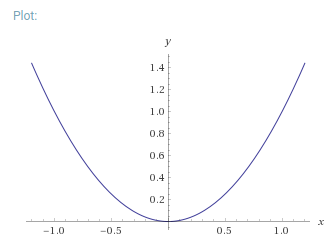
\includegraphics[width=\linewidth]{img/socp.png}
  \caption{凸関数のグラフ}
  \label{socp}
 \end{center}
\end{figure}
よって,非伸張性制約と深度最大化をSOCPとして最適化問題を解くことができる.
\begin{equation}
    \begin{aligned}
        & \underset{\bm{Q}} {\text{max}} && {\bm{p}}_3^{\mathrm{T}} \sum_{i=1}^{n_c} \bm{Q}\\
    &\text{subject to} &&
        \tiny
        \| 
        \left(
        \begin{array}{c}
          \mathrm{\bm{p}}_1^{\mathrm{T}}  \\
          \mathrm{\bm{p}}_2^{\mathrm{T}}
        \end{array} \bm{Q}_i
      \right)
      - \bm{q}_i^{\prime}\mathrm{\bm{p}}_3^{\mathrm{T}} \bm{Q}_i \| \le \varepsilon_{\mathcal{I}} \mathrm{\bm{p}}_3^{\mathrm{T}} \bm{Q}_i \normalsize &&& \forall i \in \{1, ..., n_c\}\\
    &                  && \| \bm{Q}_i -\bm{Q}_j\| \le d_{ij} \\ &&& \forall(i, j) \in \varepsilon \\
    &                  && \mathrm{\bm{p}}_3^{\mathrm{T}} \ge 0  &&&  \forall i \in \{1, ..., n_c\}
    \end{aligned}
    \label{eq:socp}
\end{equation}

\section{平滑化と非伸張性表面の推定}\label{sec:FFDref}
SOCP定式化による深度の合計の最大化問題の解は,妥当な推定結果をもたらすが,非伸張性に関する有効な原理に基づいておらずヒューリスティックな解である.
この項では,表面の非伸張性の原理に基づく定式化を提案する.
表面モデルを関数$ \mathcal{W}: \mathbb{R}^2 \to \mathbb{R}^3$ と定義する.写像$\mathcal{W}$は,テンプレート平面から3次元空間にマッピングする.
非伸張性原理とは,写像$\mathcal{W}$がどこでも局所的に等長(isometry)であるという.この制約条件はヤコビアン行列で表現することが可能である.
今,行列$\mathrm{J}(\mathrm{\bm{q}}) \in \mathbb{R}^{3 \times 3}$を,点$\mathrm{\bm{q}}$で求めたヤコビアン行列$\partial \mathcal{W} / \partial \mathrm{\bm{q}}$とする.
$\mathrm{J}(\mathrm{\bm{q}})$の列が正規直行であるならば,関数$\mathcal{W}$は点$\mathrm{\bm{q}}$において等長である.
この局所的等長性は次式の最小2乗等式条件にしたがって,表面全体に施すことが可能である.
\begin{equation}
    \iint \|\mathrm{J}(\mathrm{\bm{q}})^{\mathrm{T}}\mathrm{J}(\mathrm{\bm{q}}) - \mathrm{I}_2 \|^2 \mathrm{d\bm{q}} = 0
    \label{eq:isometry}
\end{equation}
実際には,離散点$\bm{g}$を与えるので\eqref{eq:isometry}は次式になる.
\begin{equation}
    \varepsilon_i(\mathcal{W})=\sum_{j=1}^{n_j}\|\mathrm{J}(\bm{g}_j)^{\mathrm{T}}\mathrm{J}(\bm{g}_j) - \mathrm{I}_2 \|^2
    \label{eq:isometry_orthonormal}
\end{equation}
ここで,$\{\bm{g}_j\}_{j=1}^{n_j}$は,テンプレート画像空間上の細かい規則的なグリッド上の2次元点の集合である.本研究では$30\times30$のグリドサイズを採用している.
本研究では,$\varepsilon_i$を有効な表面全てにおいて最小化する.3次元点$\mathcal{W}(\mathrm{\bm{q}}_i)$は,全ての$i$について入力画像空間の点$\mathrm{\bm{q}}_i^{\prime}$,もしくはその近くに投影される.

\subsection{表面モデルの媒介変数}
ここでは,$\varepsilon_i$を最小化する.全ての有効な表面における,\eqref{eq:isometry_orthonormal}に対して変分問題とみなす代わりに,媒介変数(parametric)の族(familey)として考える.
族とは数学用語で添字つけされた元の集まりをいう.簡単な例はmベクトルの列要素などがそれに当たる.
さて,本研究では,表面モデルを媒介変数で最小化するために,一様3次元B-Spline(uniform cubic Basis-Spline)を元にしたFFD(Free-Form Deformations)\cite{Rueckert1999}を用いる.
ここで,FFD媒介変数表示した表面モデル$\mathcal{W}_{\bm{\ell}}: \mathbb{R}^2 \to \mathbb{R}^3$であるとする.3次元点の媒介変数$\bm{\ell}_{jk}; j \in \{1, \dots, n_u\}, k \in \{1, \dots, n_v\}$であるとする.

テンプレート画像空間の点$\mathrm{\bm{q}} = (u, v)$について,3次元表面上の点は次式で与えられる.
\begin{equation}
    \mathcal{W}_{\bm{\ell}}(\mathrm{\bm{q}}) = \sum_{j=1}^{n_u}\sum_{k=1}^{n_v} \bm{\ell}_{jk}N_j(u)N_k(v)
\end{equation}
関数$N_{j},N_{k}$は,3次の多項式で表されるB-spline基底関数である.点$\mathrm{\bm{q}}_i = (u_i, v_i)$が既知で固定であるならば,3次元表面上の点$\mathcal{W}_{\bm{\ell}}(\mathrm{\bm{q_i}})$は媒介変数の点$\bm{\ell}_{jk}$の線形結合で表現される.また,$\mathcal{W}_{\bm{\ell}}(\mathrm{\bm{q_i}})$は,$\mathcal{W}_{\bm{\ell}}(\mathrm{\bm{q_i}}) = \mathrm{W}_i\bm{\ell}$と書き換えられる.
ただし,$\mathrm{W}_i$は,点$\mathrm{\bm{q}}_i$にのみ依存する$3\times n_u n_v$の行列である.また,$\bm{\ell}$は点$\bm{\ell}_{jk}$をすべて連結したベクトルである.
したがって,3次元表面上の点は媒介変数ベクトルの1次線形式で求めることができる.
多項式$N_j, N_n$は,注目点$\bm{\ell}_{jk}$の周辺の制御点にのみ依存するので,行列$\mathrm{W}_i$は疎な行列である.行列が疎である事は計算効率に重要な意味を持つ.

\subsection{最小2乗法問題における表面推定}
\eqref{eq:socp}において3次元点$Q_i$を$\mathrm{W}_i\bm{\ell}$で置き換えることによって,制約条件を次式のように書き換えられる.
\begin{equation}
    \left|\left|
    \left( 
        \left[
            \begin{array}{c}
                \mathrm{\bm{p}}_1^{\mathrm{T}}  \\
                \mathrm{\bm{p}}_2^{\mathrm{T}}
            \end{array}
        \right]
        - \bm{q}_i^{\prime}\mathrm{\bm{p}}_3^{\mathrm{T}} 
    \right)\mathrm{W}_i\bm{\ell}
    \right|\right|
    \le \varepsilon_{\mathcal{I}}\mathrm{\bm{p}}_3^{\mathrm{T}}\mathrm{W}_i\bm{\ell}
    \label{eq:constraint}
\end{equation}
\eqref{eq:constraint}を制約条件として,全ての媒介変数ベクトル$\bm{\ell}$によって\eqref{eq:isometry_orthonormal}で与えられる非伸長性のコスト関数$\varepsilon_i(\mathcal{W})$を最小化するものとして定式化できる.
\eqref{eq:constraint}は,SOCP制約であるが,コスト関数\eqref{eq:isometry_orthonormal}はパラメータにおいて次元より高い.
非線形最適化問題の困難さを回避するために,コスト関数に再投影誤差を含めることによって,困難さを解消した手法を提案する.

再投影誤差の式を簡単化するために,ここでは,補助変数として深度$\mu_i$を導入する.このとき,最小化問題は次式をとる.
\begin{equation}
    \begin{aligned}
        & \underset{\bm{\mu}, \bm{\ell}} {\text{min}} && \varepsilon_{d}(\mu, \bm{\ell}) + \alpha \varepsilon_i(\bm{\ell})+\beta\varepsilon_s(\bm{\ell})\\
    \end{aligned}
    \label{eq:evaluate}
\end{equation}
ここで,$\varepsilon_d,\varepsilon_i, \varepsilon_s$は再投影誤差のデータ,非伸長性,滑らかさを示す.
再投影誤差データの項は再構成された表面と対応点の一貫性を保証する.$\varepsilon_i$は表面の非伸張性を与え,$\varepsilon_s$はオクルージョンなどに対処するために,滑らかな表面を与える.
これらの3つの項どうしの相対的な影響は重み係数$\alpha, \beta \in \mathbb{R}_+$によって制御される.
$\mathbb{R}_+$は,正の実数空間である.
非伸張性に関してはすでに述べた.ここでは,\eqref{eq:evaluate}における$\varepsilon_d, \varepsilon_s$について述べる.

\paragraph{データ項}
\eqref{eq:cons_tmp_img}の$\bm{Q}_i$を$\mathrm{W}_i\bm{\ell}$で置き換えると,ある点に関する再投影誤差の式が得られる.しかし,結果としてデータ項は媒介変数$\bm{\ell}$に関して非線形な式となる.
\begin{eqnarray}
    \left|\left| 
    \left[
    \begin{array}{c}
      \mathrm{\bm{p}}_1^{\mathrm{T}}   \\
      \mathrm{\bm{p}}_2^{\mathrm{T}}
    \end{array}
  \right]\bm{Q}_i
 - \bm{q}_i^{\prime}\mathrm{\bm{p}}_3^{\mathrm{T}} \bm{Q}_i \right|\right|
 &\le& \varepsilon_{\mathcal{I}}\mathrm{\bm{p}}_3^{\mathrm{T}} \bm{Q}_i \nonumber\\
    \left|\left| 
    \left[
    \begin{array}{c}
      \mathrm{\bm{p}}_1^{\mathrm{T}}   \\
      \mathrm{\bm{p}}_2^{\mathrm{T}}
    \end{array}
  \right]\mathrm{W}_i\bm{\ell}
 - \bm{q}_i^{\prime}\mathrm{\bm{p}}_3^{\mathrm{T}} \mathrm{W}_i\bm{\ell} \right|\right|
 &\le& \varepsilon_{\mathcal{I}}\mathrm{\bm{p}}_3^{\mathrm{T}} \mathrm{W}_i\bm{\ell}
 \label{eq:cons_tmp_replace}
\end{eqnarray}
ここで,補助変数深度$\mu$を用いて\eqref{eq:cons_tmp_replace}を次式のようになる.
\begin{equation}
    \varepsilon_d(\bm{\mu},\bm{\ell}) = \sum_{i=1}^{n_c} \|\mathcal{W}_{\ell}(\mathrm{\bm{q}}_i) - \mu_i\mathrm{P}^{-1}\overline{\mathrm{\bm{q}}}_i^{\prime} \|^2
    \label{eq:3derror}
\end{equation}
データ項は,表面上の点$\mathcal{W}_{\ell}$と,点$\mathcal{W}_{\ell}$と$\mathrm{\bm{q}}_i$で定義できるカメラの光学線上を動く奥行き$\mu_i$の点との間の距離を求めることになる.

\paragraph{平滑化項}
場合によっては、点の対応と非伸縮性表面の仮説は十分ではない。
例えば、表面の角に点の対応がない場合、表面の振る舞いを定義することができない.
表面は伸縮しない限り,どのような変形もありうる.
そこで,オクルージョンのようなケースに対処するため,平滑化項を定義する.
通常,平滑化項はアンダーフィッティングやオーバーフィッティングの望ましくない影響を緩和するために使用する.また,平滑化項にかかる重み係数は適切な値を設定する必要がある.
ただし,本研究は非伸張特性による制約条件を用いているため,特に重要視する必要がない.したがって,係数は小さな値を適用する.しかし,無視できないほどには大きな値を用いる.例えば,$\beta = 10^{-4}$である.
平滑化項は,曲げエネルギーを用いて次式に定義する.
\begin{equation}
    \varepsilon_s(\bm{\mu}, \bm{\ell}) = \sum_{i=1}^3 \iint \left|\left| \frac{\partial^2\mathcal{W}_{\bm{\ell}}^i(\mathrm{\bm{q}})}{\partial\mathrm{\bm{q}}^2} \right|\right|_{\mathcal{F}}^2 \mathrm{d \bm{q}}
\end{equation}

ここで,$\mathcal{W}_{\bm{\ell}}^i(\mathrm{\bm{q}})$は$i$番目の点を,$\|\cdot\|_\mathrm{F}$はヘッセ行列のフロベニウスノルムである.
行列の全成分の2乗和の平方根をフロベニウスノルムという.
ヘッセ行列とは,2階の変動関数を並べた行列である.
\begin{equation}
    H(\mathcal{W}_{\bm{\ell}}^i(u,v))=
    \left[
        \begin{array}{c c}
            \frac{\partial^2\mathcal{W}_{\bm{\ell}}^i(u,v)}{\partial u^2} & \frac{\partial^2\mathcal{W}_{\bm{\ell}}^i(u,v)}{\partial u \partial v}  \\
            \frac{\partial^2\mathcal{W}_{\bm{\ell}}^i(u,v)}{\partial u \partial v} & \frac{\partial^2\mathcal{W}_{\bm{\ell}}^i(u,v)}{\partial v^2}
        \end{array}
    \right]
\end{equation}
FFDより,$\varepsilon_s$はシンプルな線形閉形式(linear closed-form expression)で表せる
四則演算と初等関数の合成による解の表し方を閉形式という.
\begin{equation}
    \varepsilon_s(\bm{\ell}) = \|\mathrm{B}^{1/2}\bm{\ell}\|^2 = \bm{\ell}^{\mathrm{T}}\mathrm{B}\bm{\ell}
\end{equation}

ここで,$\mathrm{B} \in \mathbb{R}^{3p\times3p}$は,B-spline基底関数の2次導関数から計算した,半正定値行列である.
行列$A \in \mathbb{R}^{n\times m}$の対称行列がベクトル$\forall \mathrm{\bm{x}}$に対して,
\begin{equation*}
    \mathrm{\bm{x}}^{\mathrm{T}} A \mathrm{\bm{x}} \geq 0
\end{equation*}
を満たすとき,$A$を半正定値行列という.

\paragraph{初期解}
\eqref{eq:evaluate}の問題は,LM(Levenberg-Marquardt)法のような反復施行することで慣例的に解くような非線形最小2乗最小化問題である.通常,このような問題では,初期値を要する.
本研究は,項\ref{sec:socp}で求めた3次元点にFFDの表面をフィッティングし,さらに,そのパラメータに関して,最小二乗法を解くことにより,初期パラメータ$\bm{\ell}$を得る.
\begin{equation}
    \underset{\bm{\ell}} {\text{min}} {\sum_{i=1}^{n_c}\|\mathcal{W}_{\bm{\ell}}(\mathrm{\bm{q}}_i)-\bm{Q}_i\|^2} \iff \underset{\bm{\ell}} {\text{min}} {\sum_{i=1}^{n_c}\|\mathrm{W}_i\bm{\ell}-\bm{Q}_i\|^2}
\end{equation}
%% 参考文献
\bibliographystyle{sieicej}
\bibliography{library}%bibTexのファイル名
%\begin{thebibliography}{99}
%%\bibitem{bib:Latex2E}
%%奥村晴彦,改定第4版 LATEX2$\varepsilon$ 美文書作成入門,\\須藤真己(編),pp.1-184,(社)技術評論社,東京,2007.
%\end{thebibliography}


\end{document}
